	\begin{frame}
	\frametitle{День 2. 19 августа}
	\framesubtitle{д.р. Кичкинакол Уллукёльский~--- оз. Гитче-Кёль~---оз. Уллу-Кёль} % Optional subtitle
	\begin{columns}[c] % The "c" option specifies centered vertical alignment while the "t" option is used for top vertical alignment
		\begin{column}{0.45\textwidth} % Left column width
			\begin{itemize}
				\item Забег по долине Кичкинакола
				\item Купание в Гитче-Кёль и думы руководы
				\item Попытки в снежные занятия
				\item ...Последнее, что видит дрон~--- это снежник Уллукёля Восточного \frownie
				\item Прошли \textbf{5.6} км
				\item ЧХВ: 3:25
				\item Набор/сброс: \textcolor{darkred}{\textbf{+650}}/\textcolor{darkblue}{\textbf{-0}}~м
			\end{itemize}
			
		\end{column}
		\begin{column}{0.5\textwidth} % Right column width
			\centering
			\includegraphics[width=\linewidth]{../pics/mini_maps/19}
		\end{column}
	\end{columns}
\end{frame}


\begin{frame}
	\frametitle{Дорога до озёр и далее на перевал}
	\framesubtitle{День 2, 19 августа}
	\centering
	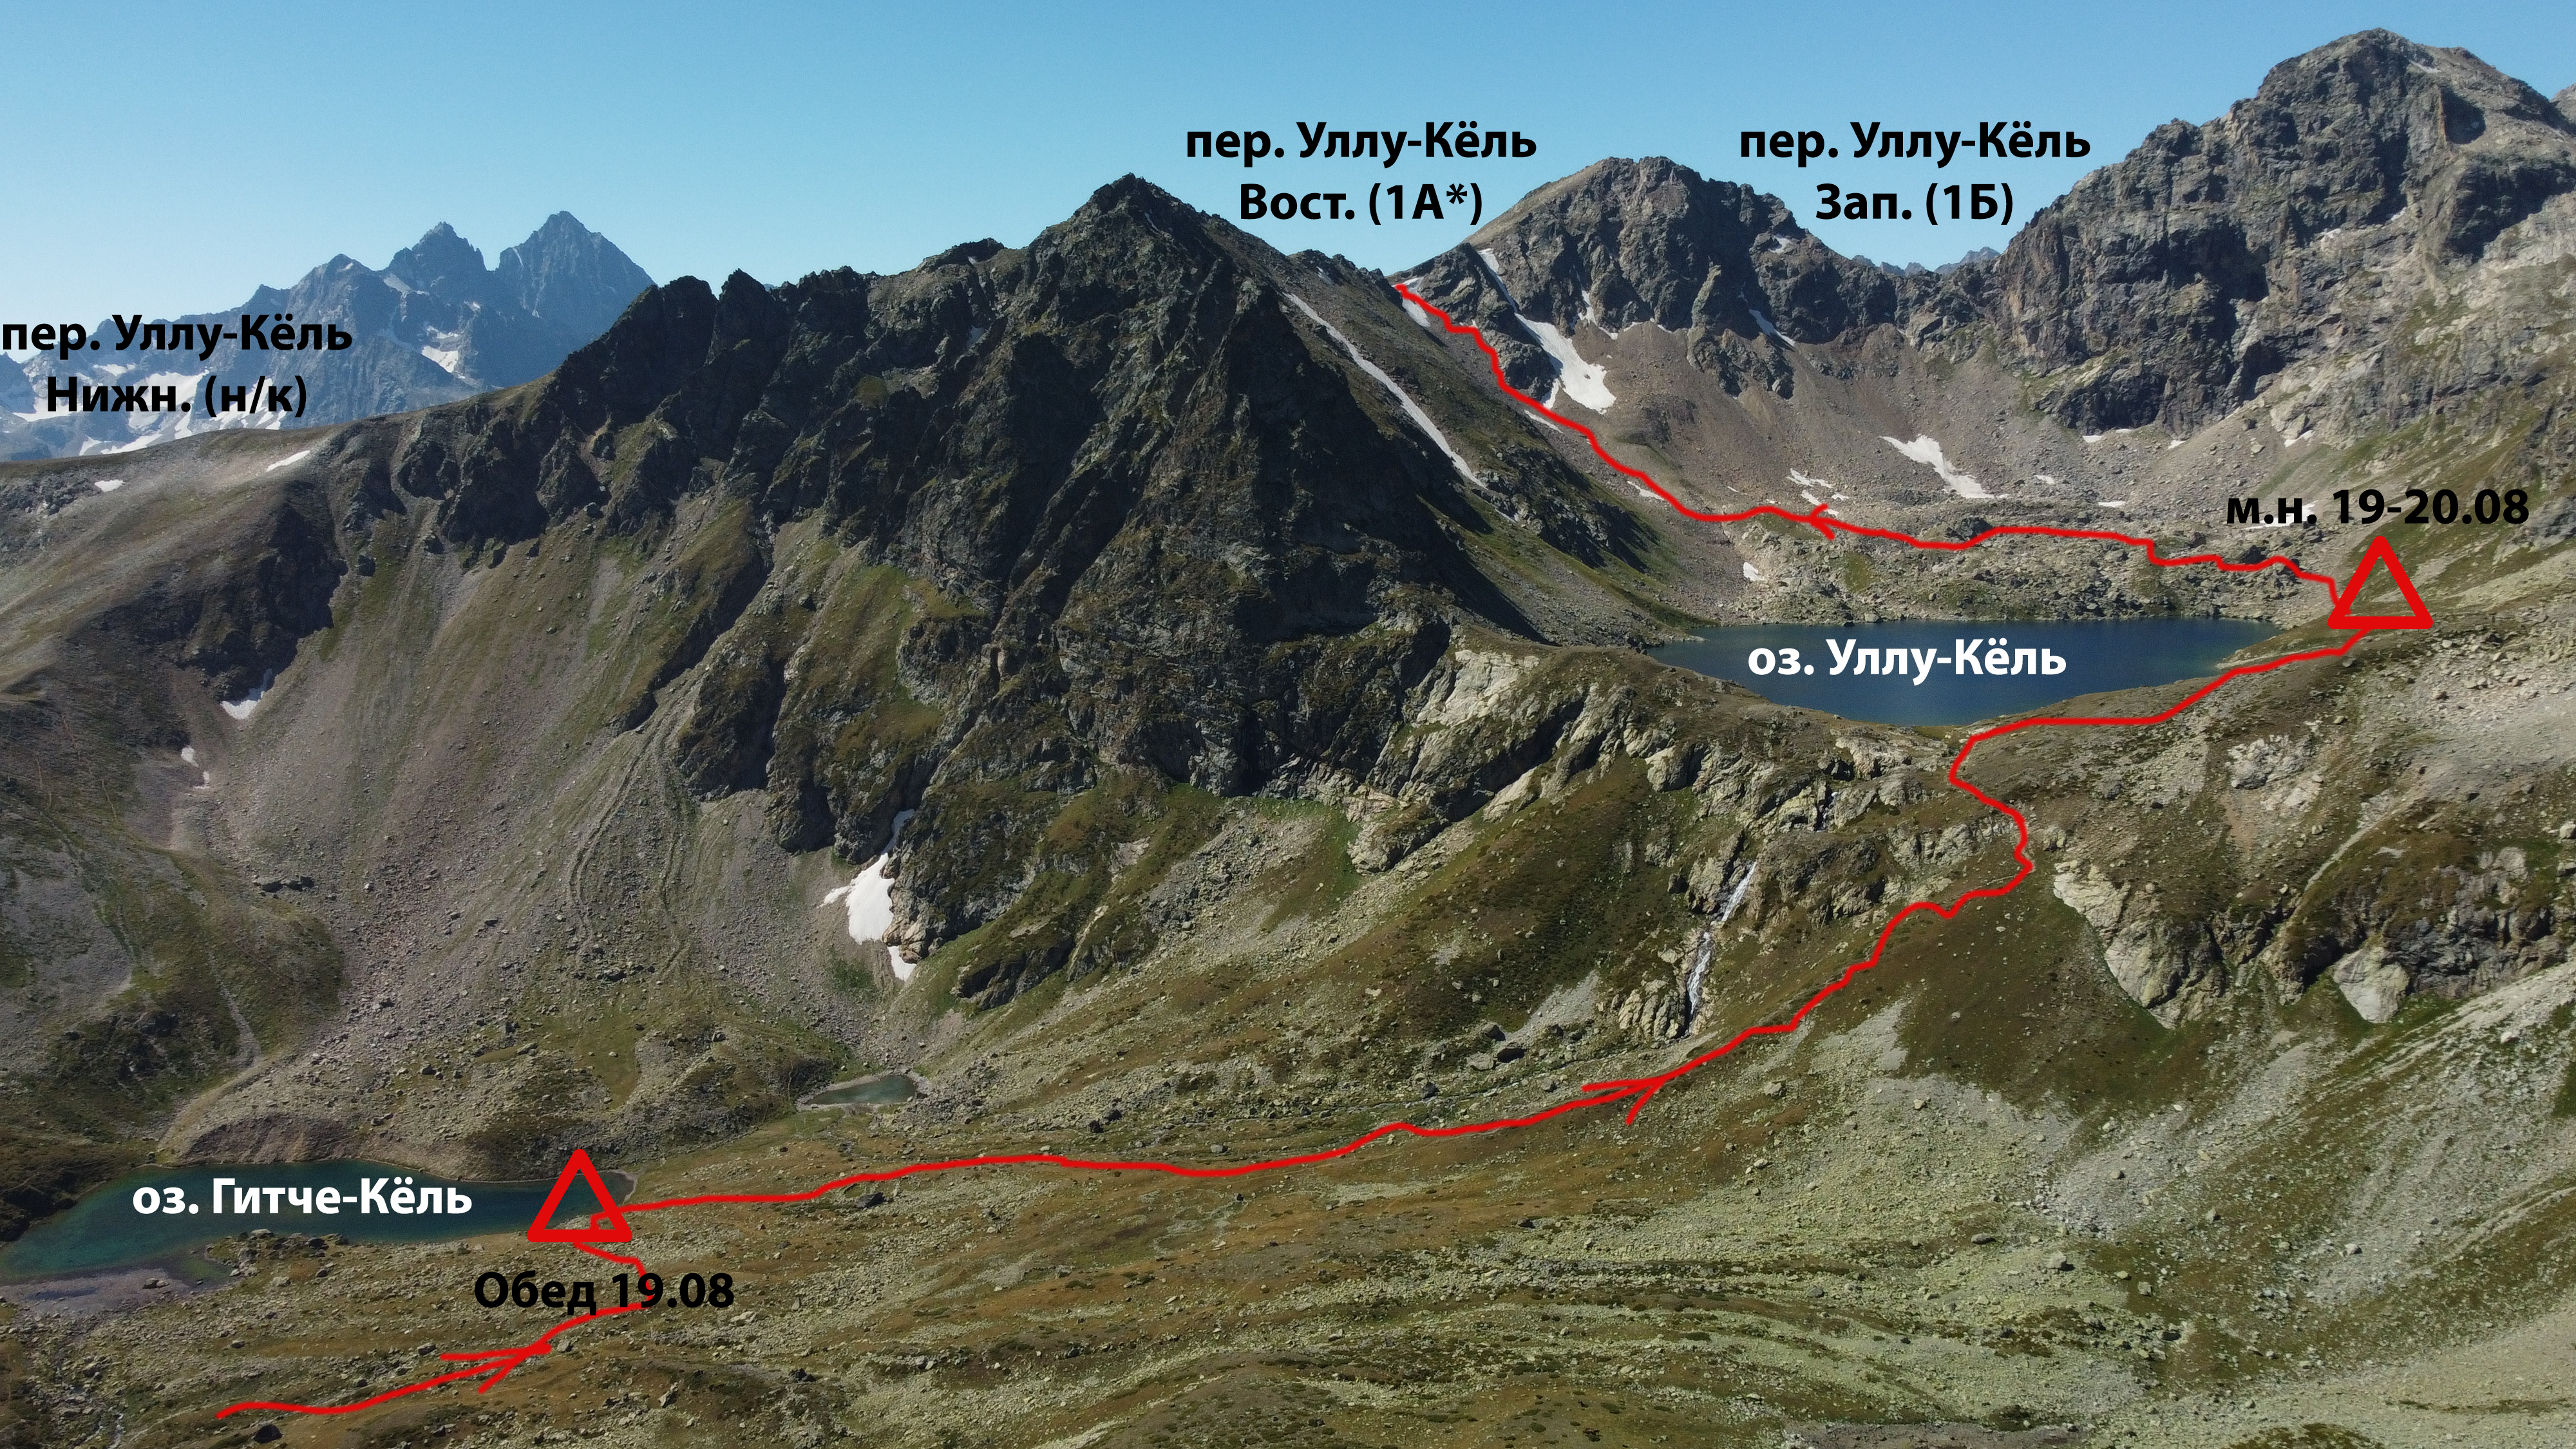
\includegraphics[width=\linewidth]{../pics/ullu_kuel_route}
\end{frame}